% vim: et sw=2 ts=2 sts=2

\section{Análise das Possíveis Abordagens}
\frame{
  \frametitle{Análise das Possíveis Abordagens}
  \begin{block}{}

    %\begin{enumerate}
    %  \item Lógica Fuzzy
    %  %\item CRF + ACO/SA
    %  \item Rede Neural
    %\end{enumerate}

    \begin{table}
      \begin{center}
        \begin{tabular}{|c|c|c|c|c|c|}
          \hline
          Critério          & ACO & SA  & L. Fuzzy & ANN\\
          \hline
          Requer modelo     & Sim & Sim &   Sim    & Não\\
          de classificação  &     &     &          &    \\
          \hline
          Estrutura de      & Sim & Sim &   Sim    & Não\\
          fácil análise     &     &     &          &    \\
          \hline
          Degradação devido & Sim & Não &   Não    & Não\\
          a discretização   &     &     &          &    \\
          \hline
          Fácil             & Não & Não &   Não    & Sim\\
          pré-processamento &     &     &          &    \\
          \hline
          Fácil             & Não & Não &   Não    & Sim\\
          pós-processamento &     &     &          &    \\
          \hline
          Característica    & Modelo   & Parte das & Parte das    & Somente    \\
          reutilizável      & treinado & regras    & regras       & topologia  \\
          \hline
        \end{tabular}
        \caption{Tabela comparativa dos métodos}
        \label{table:metodos}
      \end{center}
    \end{table}

  \end{block}
}

\frame{
  \frametitle{Análise das Possíveis Abordagens}
  \scriptsize
  \lstinputlisting{../train.log}
}

\frame{
  \frametitle{Análise das Possíveis Abordagens}
  \begin{block}{}
    \begin{figure}[thpb]
      \centering
      \begin{subfigure}[b]{0.49\textwidth}
        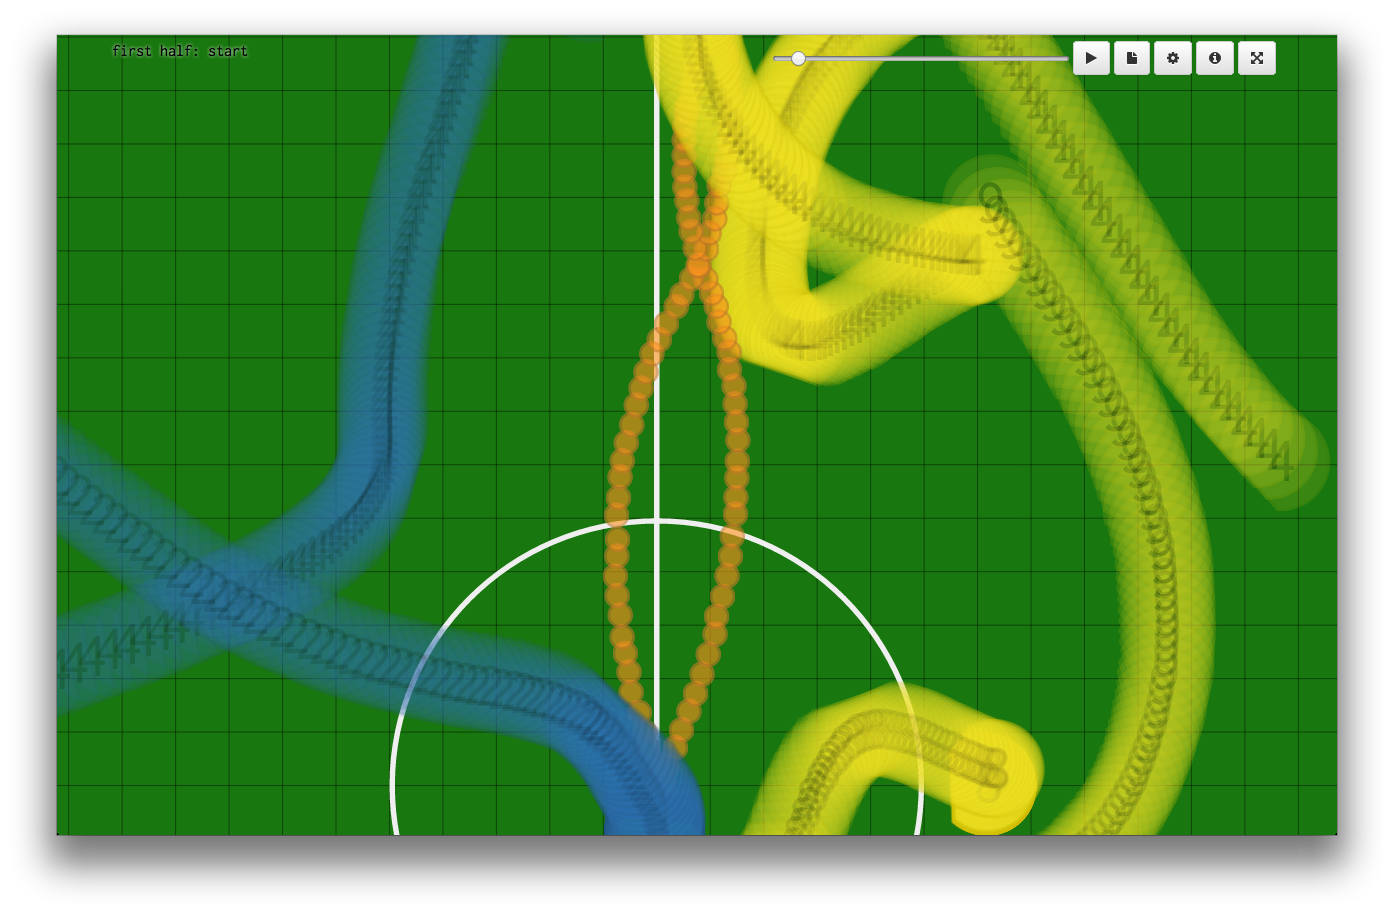
\includegraphics[width=\textwidth]{figuras/log_rastro.png}
        \caption{Rastro duplo divergente}\label{fig:log_rastro}
      \end{subfigure}
      \begin{subfigure}[b]{0.49\textwidth}
        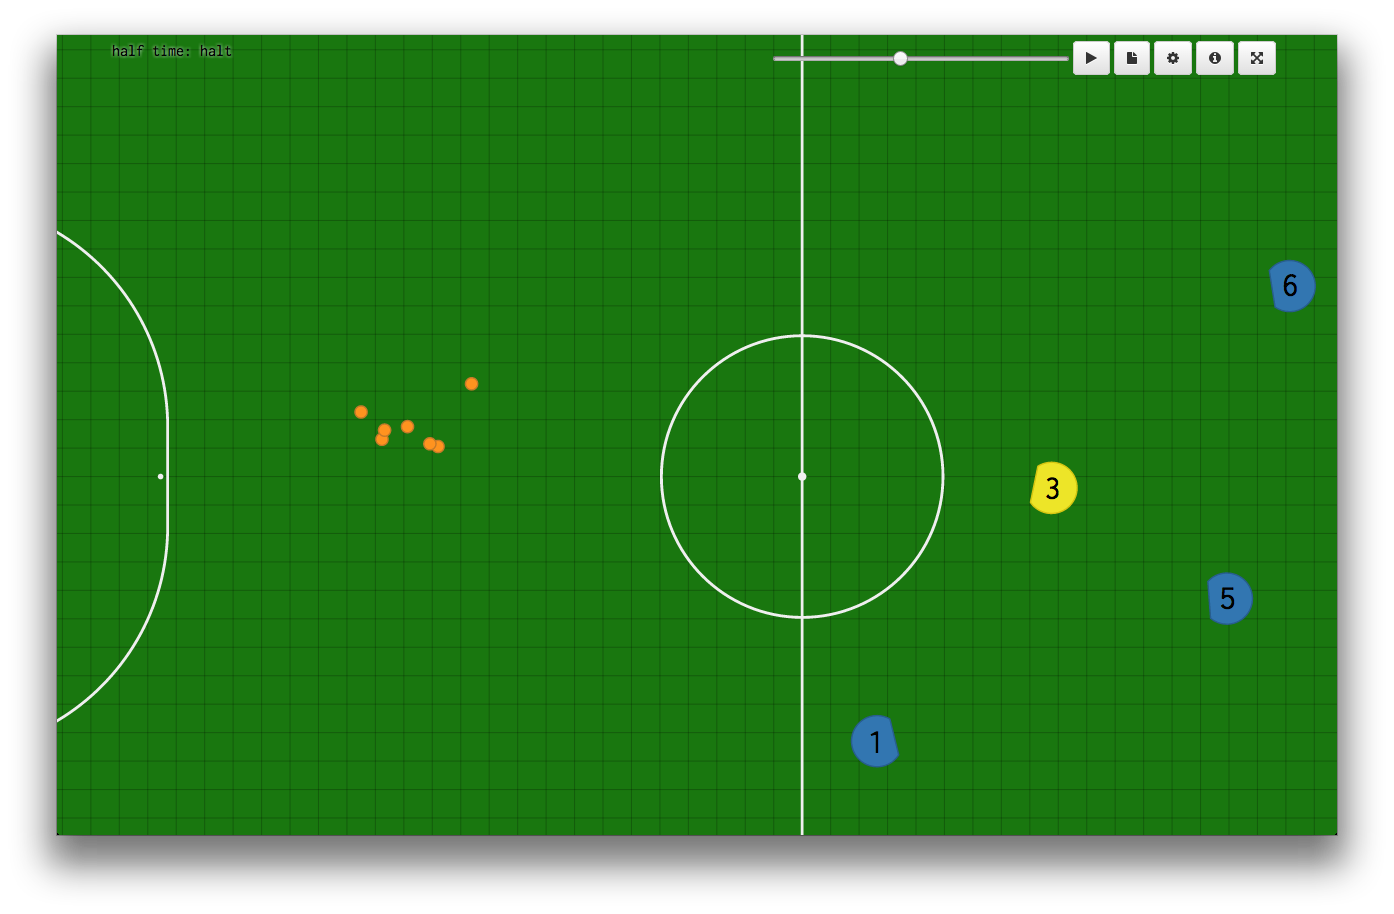
\includegraphics[width=\textwidth]{figuras/log_multi.png}
        \caption{Objetos "fantasmas"}\label{fig:log_multi}
      \end{subfigure}
      \caption{Análise dos logs.}\label{fig:logs}
    \end{figure}
  \end{block}
}
